\documentclass[11pt]{article}
\usepackage[utf8]{inputenc}
\usepackage[T1]{fontenc}
\usepackage{amsmath}
\usepackage{amsfonts}
\usepackage{amssymb}
\usepackage{makeidx}
\usepackage{graphicx}
\usepackage{lmodern}
\usepackage{subfigure}
\usepackage{kpfonts}
\usepackage{caption}

\author{262719}
\title{\begin{huge}
Linear Models
\end{huge}\\Data Analysis Project}
\date{}
\begin{document}
\maketitle
 
\tableofcontents
\newpage

\section{Introduction}

	The goal of this report is to discuss the factors affecting the concentration of prostate specific antigen (PSA). We will base our analysis on the dataset published in Journal of Urology 141(5), 1989, pp 1076-1083. The datasets contain 8 variables and 97 observations and was collected on men before they underwent radical prostatectomy. We will first describe the methods that we will use and then construct a Gaussian linear model for the data. We will then discuss the results and the strengths and weaknesses of the approach. Finally we will propose improvements for further investigations

\section{Methodology}

	We will first fit a Gaussian linear model to the data with the PSA as the response while incorporating all possible covariates and then check with diagnostic plots that the 4 assumptions inherent to this model hold in this context: namely linearity, homoskedasticity, and the independence and gaussianess of the error terms. We will also look for leverage points and outliers aswell as try to assess the colinearity of the data.
	Once this done we will fit all possible models corresponding to all different combinations of covariates and select the model which has the lowest Bayesian Information Criterion (BIC). We will also build a model with backward selection. Once this done we will add interactions between the covariates selected and then compare all models produced. We will then select the final model by comparing several metrics: their Akaike Information Criterion (AIC), their BIC, the Variance Inflation Factors of their respective parameters (VIF) and their adjusted R squared.
	Finally we will interpret our results and critize them.

\section{Discussion}

	Let's start with a matrix scatterplot of the data to see if a Gaussian linear model is appropriate for the data and if transformation of covariates are needed.

\begin{figure}[htb]
\begin{center}
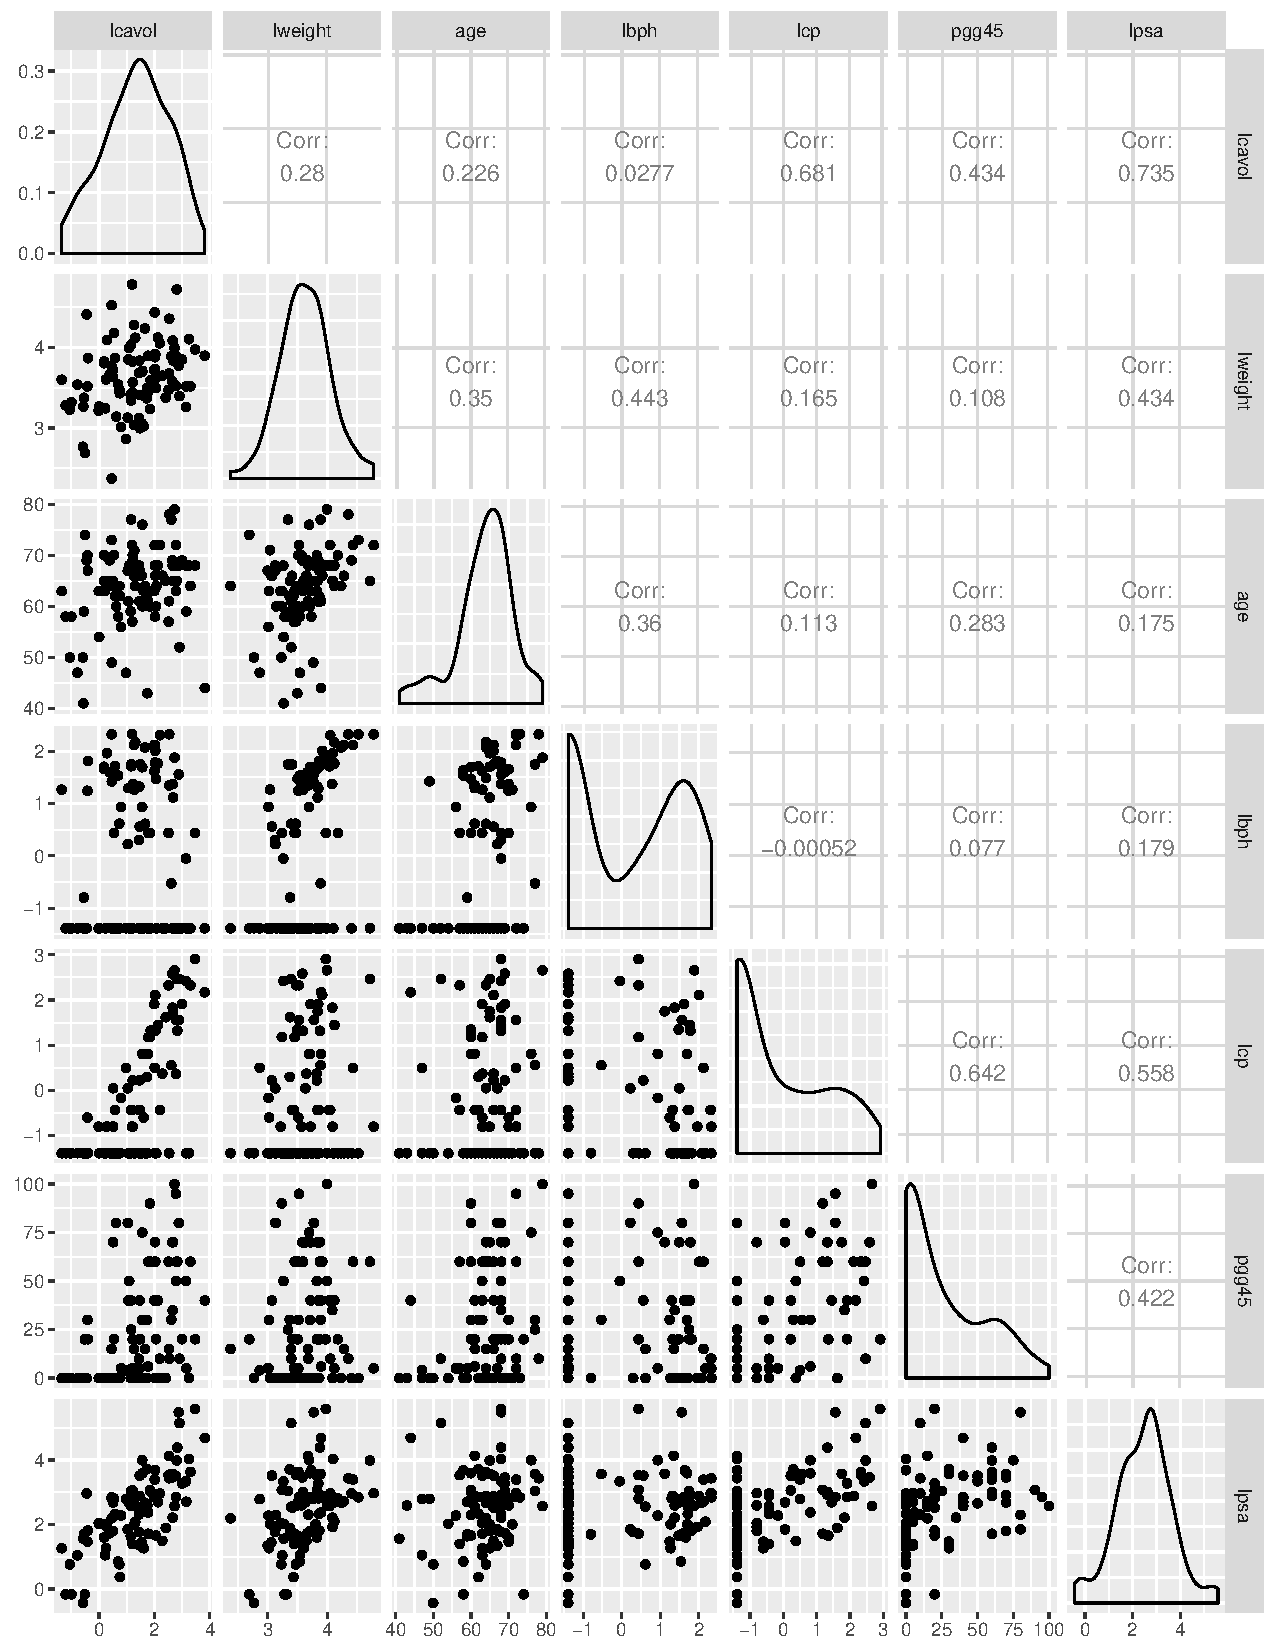
\includegraphics[height=4in,width=5in]{matrixscatterplot.pdf}
\caption{Matrix scatterplot of all covariates}
\end{center}
\end{figure}
As we can see on Figure 1 a Gaussian linear model seems appropriate to model the relationship between the explanatories and the response. We can also see that no further transformations of the covariates are needed. Further explanatory data analysis shows that there is exactly one observation with a gleason score of 8, which we will remove since it can significantly impact the fit.
	Next we verify that the hypotheses associated with the Gaussian linear model hold by looking at the plots in Figure 2

\begin{figure}[htb]
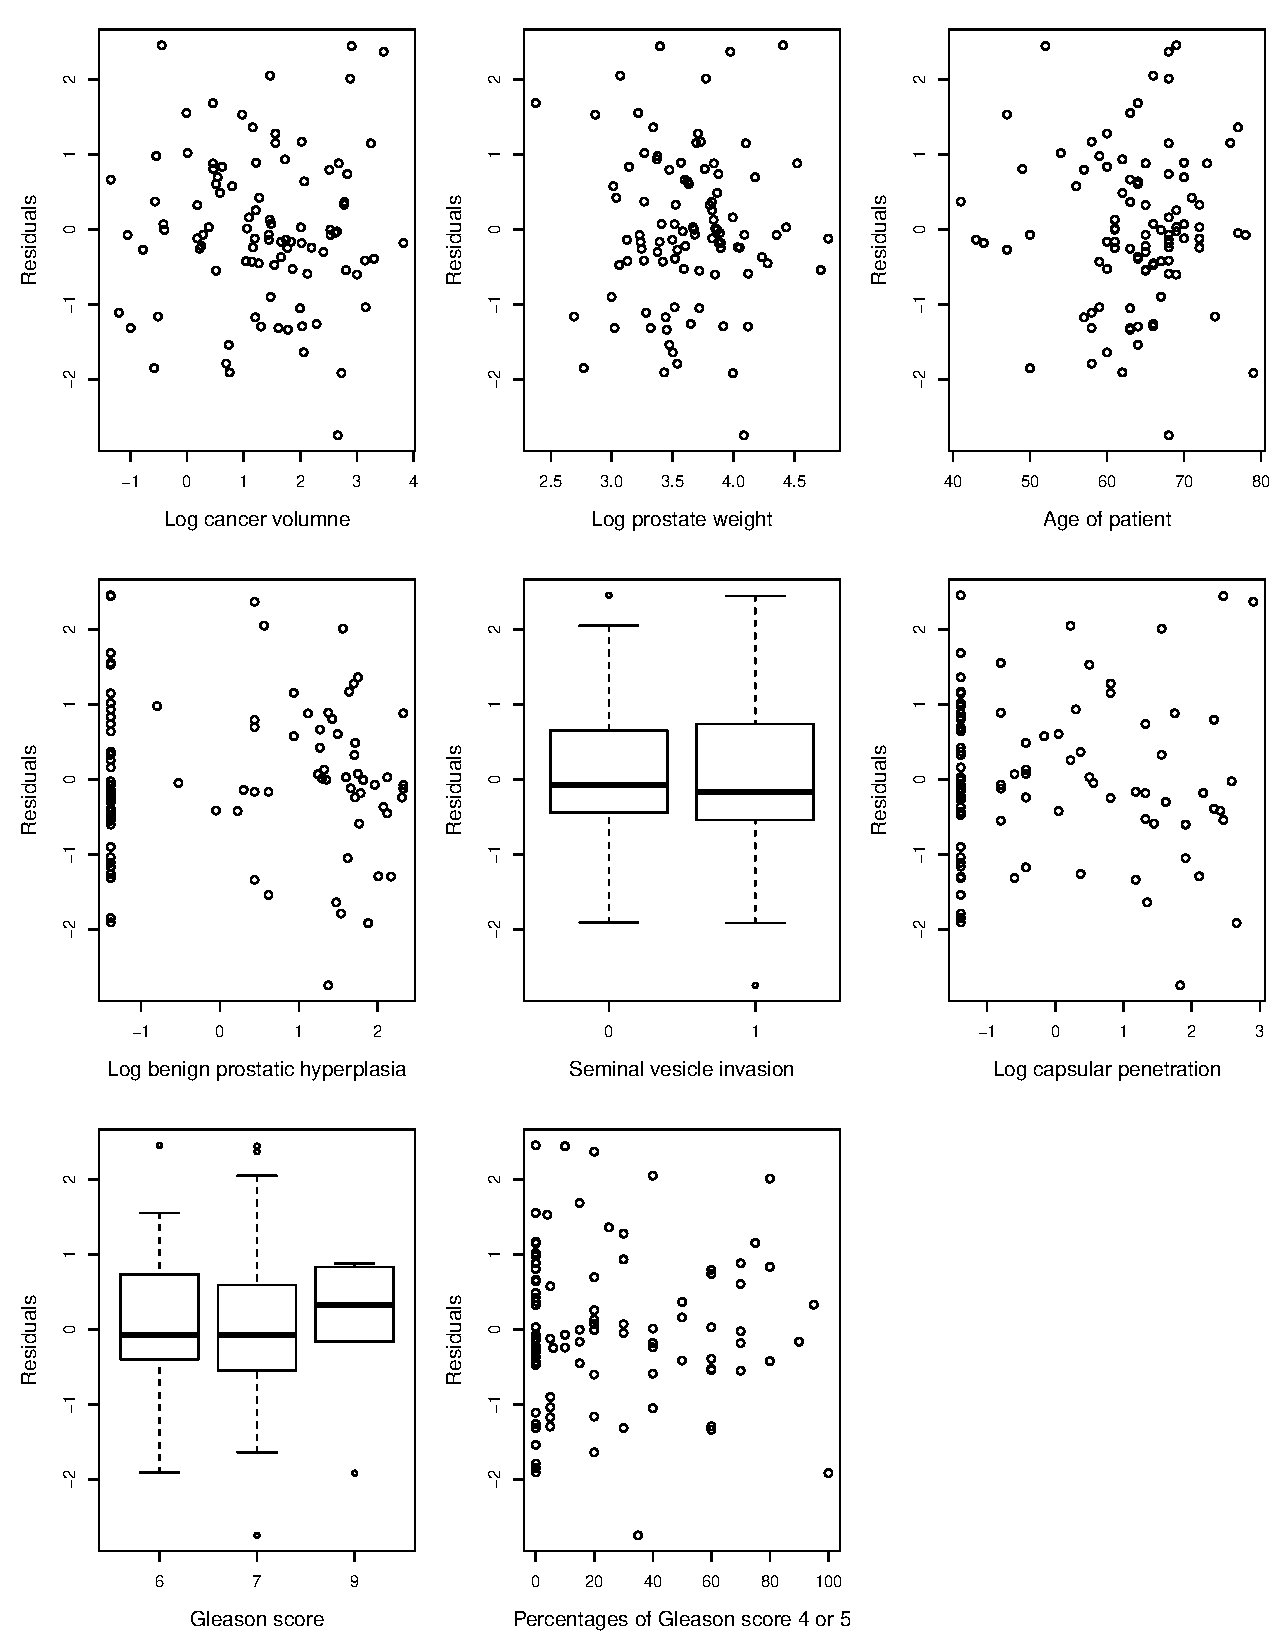
\includegraphics[height=5in,width=5in]{plspls.pdf}
\caption{Residuals vs covariates}
\end{figure}


\end{document}